\section{Simulaciones y experimentos}
    En esta sección se realizarán simulaciones y comparaciones entre distintos sistemas. Para demostrar la idea básica de sistema TIIR, se comenzerá examinando el sistema tal que

    \begin{equation}
      H(z) = \frac{z^{2}}{z^{2} - 1.9 \: z + 0.98} = \frac{B^{+}(z)}{A^{+}(z)}
    \end{equation}

    el cual se deseará truncar luego de un $N = 300 \: [\text{muestras}]$ arbitrario; esto es, se desea obtener una respuesta FIR de 301 pasos. Se comienza entonces formando el polinio de cancelación de cola como en la Eq. \ref{eq:25}, realizando división sintética de $z^{N} \: B(z)$  por $A(z)$, lo que resulta en el resto

    \begin{equation}
      B^{\prime +}(z) = - 0.162126 \: z + 0.13977
    \end{equation}

    De esta manera, se puede definir $H_{FIR}^{+}(z)$ según la Ec. \ref{eq:42}

    \begin{align}
      H_{FIR}^{+}(z) =& \frac{B(z) - z^{-N} \: B^{\prime + }(z)}{A(z)} \nonumber \\
      =& \frac{z^{2} + z^{-N} \: \left( - 0.162126 \: z + 0.139977 \right)}{z^{2} - 1.9 \: z + 0.98}
    \end{align}

    Entonces, se definen los coeficientes de $H_{FIR}^{+}(z)$  como

    \begin{itemize}
      \item $a = 0.162126$
      \item $b = 0.139977$
      \item $p = 1.9$
      \item $q = 0.98$
    \end{itemize}

    Así, se obtiene la FT de forma de llegar a un polinomio con el formato para graficar en GNU Octave

    \begin{align}
      H_{FIR}^{+}(z) =& \frac{z + a \: z^{-(N-1)} - b \: z^{-N}}{z^{2} - p \: z + q} \nonumber \\
      =& \frac{z^{2} + z^{-(N-1)} \: \left(a - b \: z^{-1} \right)}{z^{2} - p \: z + q} \nonumber \\
      =& \frac{z^{2} + \frac{a - b \: z^{-1}}{z^{N-1}}}{z^{2} - p \: z + q} \nonumber \\
      =& \frac{z^{N+1} + \left( a - b \: z^{-1} \right)}{z^{N-1} \: \left( z^{2} - p \: z + q \right)}
    \end{align}

    Ahora, si se desarrolla el término $b \: z^{-1}$

    \begin{align}
      H_{FIR}^{+}(z) =& \frac{z^{N+1} + a - \nicefrac{b}{z}}{z^{N-1} \: \left( z^{2} - p \: z + q \right)} \nonumber \\
      =& \frac{z^{N+2} + a \: z - b}{z^{N} \: \left( z^{2} - p \: z + q \right)} \nonumber \\
      =& \frac{z^{N+2} + a \: z - b}{z^{N+2} - p \: z^{N+1} + q \: z^{N}}
      \label{eq:03-00-hfir+}
    \end{align}

    Queda definida entonces la FT $H_{FIR}^{+}(z)$, y se puede insertar en GNU Octave con el algoritmo que se muestra en el algoritmo a continuación

    \lstinputlisting[language=Octave]{../code/tiir_hfir1.m}

    \begin{figure}
      \centering
      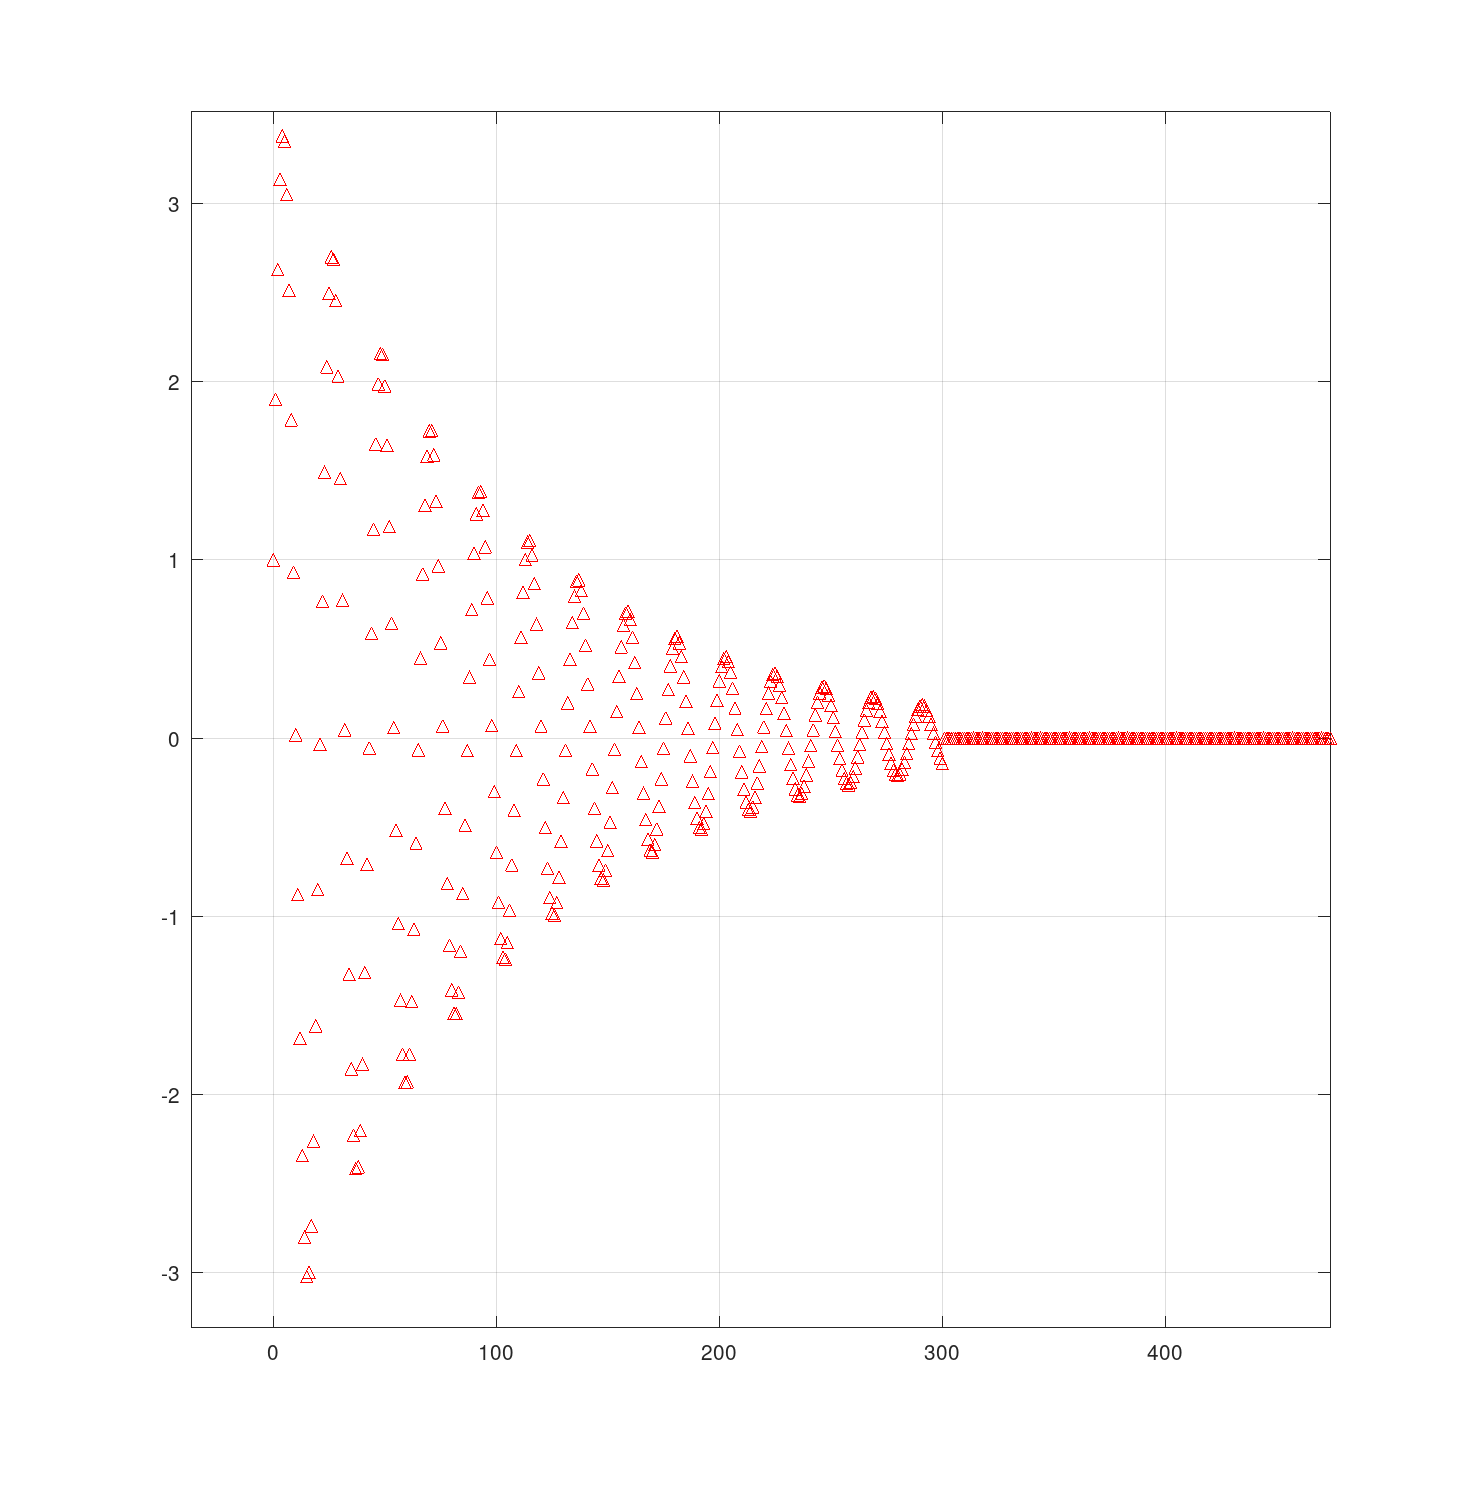
\includegraphics[width=0.52\textwidth]{../images/03-00-hfir+.png}
      \caption{Respuesta al impulso TIIR de $H_{FIR}^{+}$ según la Ec. \ref{eq:03-00-hfir+}}
      \label{fig:03-00-hfir+}
    \end{figure}

    En la Fig. \ref{fig:03-00-hfir+} se puede observar la respuesta al impulso de $H_{FIR}^{+}(z)$, donde se puede notar que efectivamente, en el paso $n=301$, la cola de la respuesta se ha subtraído.

    A continuación, se forma el sistema reverso conjugado $H_{FIR}^{-}(z)$ como se describe en la Ec. \ref{eq:47}, y se llega a

    \begin{align}
      H_{FIR}^{-}(z) =& \frac{-z \: B^{\prime -}(z) + z^{-N} \: B^{-}(z)}{A^{-}(z)} \nonumber \\
      =& \frac{-0.13977 \: z^{2} + 0.162126 \: z - z^{-N}}{0.98 \: z^{2} - 1.9 \: z +1} \nonumber \\
      =& \frac{-0.142622 \: z^{2} + 0.165435 \: z - 1.0220408 \: z^{-N}}{z^{2} - 1.938776 \: z + 1.020408}
    \end{align}

    Por lo que se pueden definir los coeficientes de $H_{FIR}^{-}(z)$ como

    \begin{itemize}
      \item $c = 0.142622$
      \item $d = 0.165435$
      \item $e = 1.020408$
      \item $u = 1.938776$
      \item $v = 1.020408$
    \end{itemize}

    Luego, se reescriben los polinomios de $H_{FIR}^{-}(z)$ de forma que sea posible computarla con GNU Octave, al igual que se realizó para $H_{FIR}^{+}(z)$

    \begin{align}
      H_{FIR}^{-}(z) =& \frac{-c \: z^{2} + d \: z - \nicefrac{e}{z^{N}}}{z^{2} - u \: z + v} \nonumber \\
      =& \frac{-c \: z^{N+2} + d \: z^{N+1} - e}{z^{N} \: \left( z^{2} - u \: z + v \right)} \nonumber \\
      =& \frac{-c \: z^{N+2} + d \: z^{N+1} - e}{z^{N+2} - u \: z^{N+1} + v \: z^{N}}
      \label{eq:03-00-hfir2}
    \end{align}

    Y se realiza entonces con la misma el algoritmo en GNU Octave como se muestra a continuación

    \lstinputlisting[language=Octave]{../code/tiir_hfir2.m}

    \begin{figure}
      \centering
      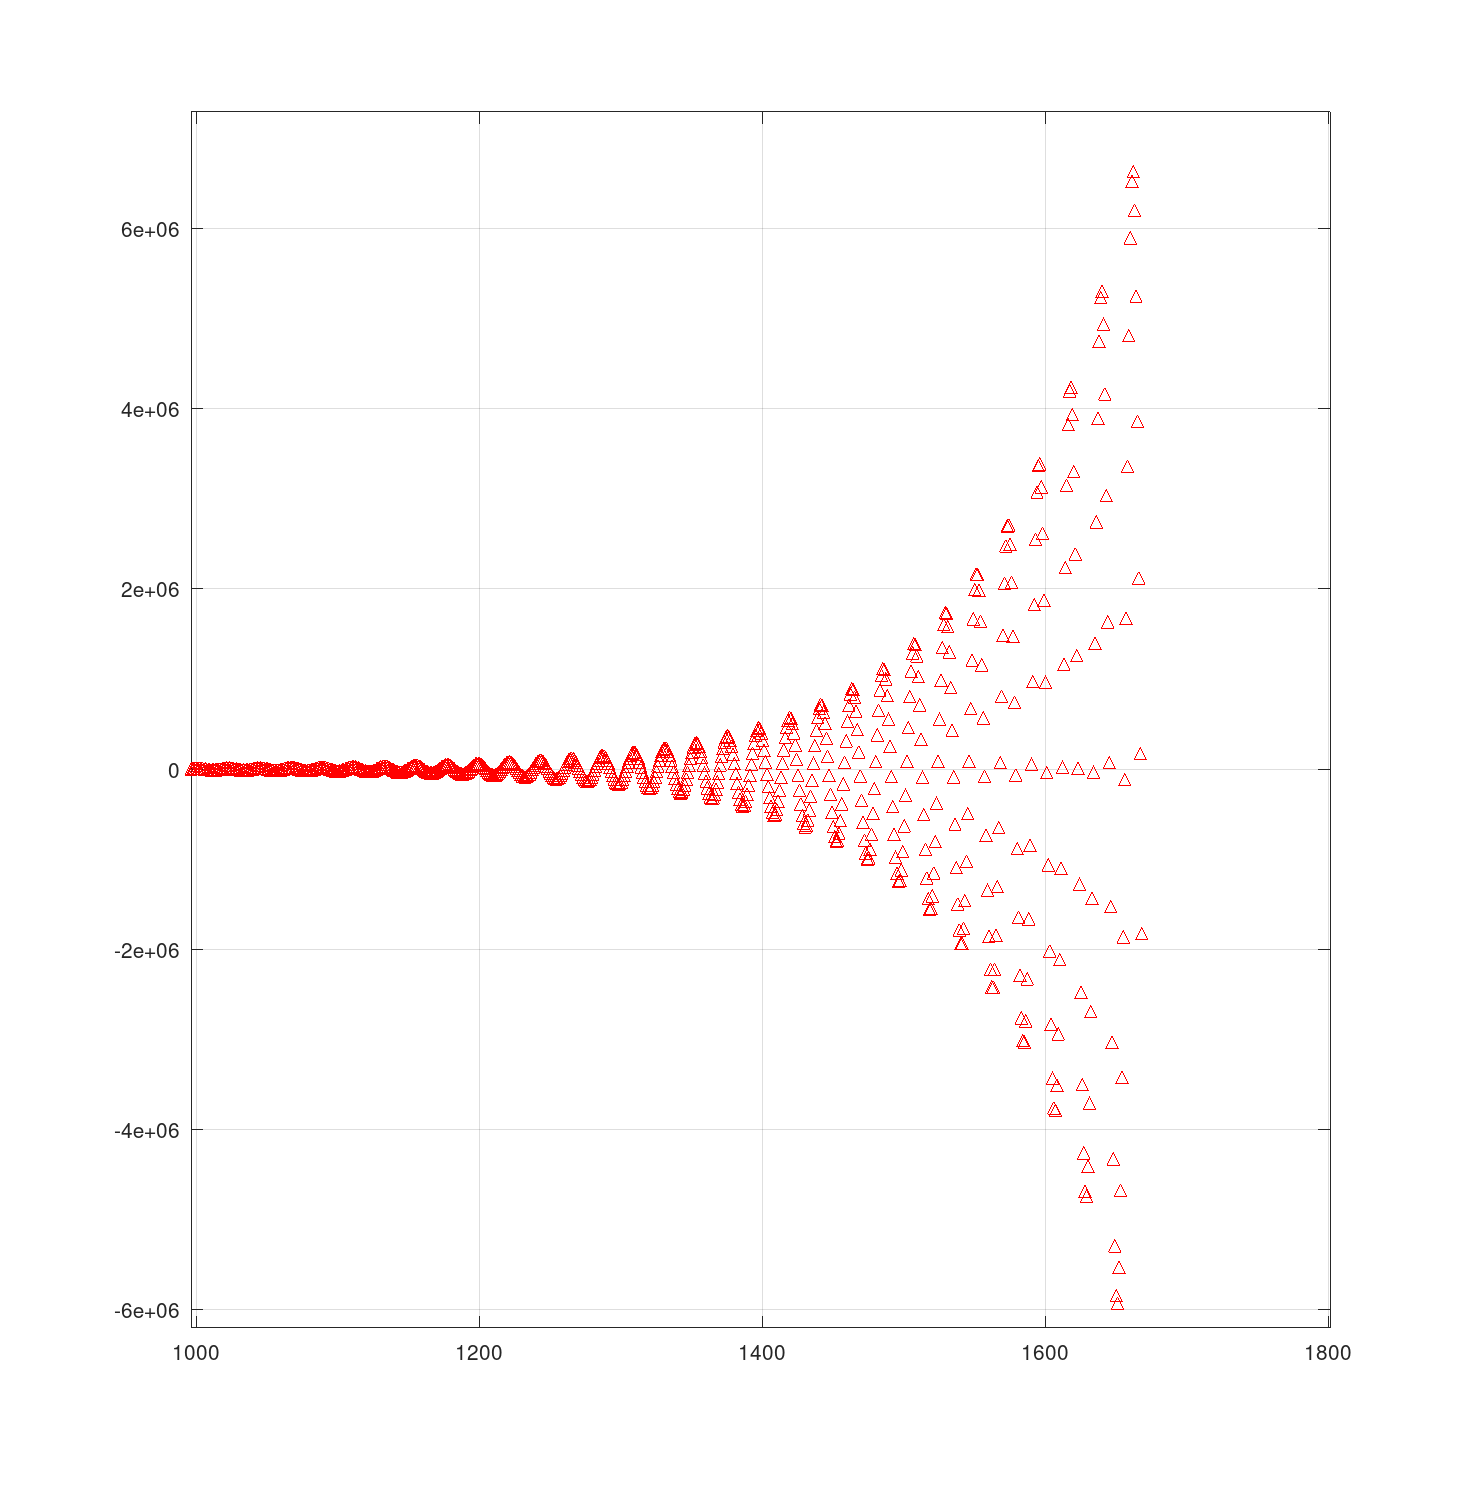
\includegraphics[width=0.5\textwidth]{../images/tiir_hfir2.png}
      \caption{Respuesta al impulso TIIR de $H_{FIR}^{-}$ según la Ec. \ref{eq:03-00-hfir2}}
      \label{fig:tiir_hfir2}
    \end{figure}

    Entonces, como se puede observar en la Fig. \ref{fig:tiir_hfir2}, el sistema posee modos ocultos inestables. Se nota que, al igual que $H_{FIR}^{+}(z)$, la cola se cancela, pero sin embargo aquí el ruido de cuantización es tan grande que eventualmente abruma a la señal.

    \subsection{Diseño de un filtro elíptico FFIR}
    Se ilustrará a continuación un filtro pasa-bajos de fase lineal FFIR
    utilizando la técnica de diseño de magnitud cuadarada como se desarrolló en
    la Sec. \ref{sec:02-02-mag-cuad}. Entonces, se deseará que el filtro cumpla
    con los siguientes criterios de diseño


    \begin{enumerate}
      \item Banda de paso normalizada $(0.00,0.10)$ en fracciones de
            $\nicefrac{f_{s}}{2}$ con al menos $0.08 \: [\unit{dB}]$ de ripple
            máximo pico-a-pico, donde $f_{s}$ se define como la frecuencia de
            muestreo.
      \item Banda de parada normalzada $(0.11,1.00)$ con al menos
            $50 \: [\unit{dB}]$ de atenuación.
      \item Fase lineal.
      \item Amplitud máxima de $\mu = 1.0$.

    \end{enumerate}

    Debido a la banda de transición angosta en el intervalo $(0.10,0.11)$, se
    selecciona un filtro elíptico como la base del diseño. Luego, 3) será
    irrelevante ya que un filtro FIR basado en la metodología TIIR (FFIR) tendrá
    las características intrínsecas de fase lineal. De esta forma, como
    observa en el algoritmo que se muestra a continuación, se pueden ingresar
    los parámetros del filtro en GNU Octave y mediante la función
    \lstinline|ellip| se obtendrán los coefientes del filtro

    \lstinputlisting[language=Octave]{../code/ellip-coeffs.m}

    \begin{itemize}
      \item $a_{0} = 1.0000$
      \item $a_{1} = -5.2007$
      \item $a_{2} = 11.4639$
      \item $a_{3} = -13.6841$
      \item $a_{4} = 9.3190$
      \item $a_{5} = -3.4305$
      \item $a_{6} = 0.5332$
    \end{itemize}

    \begin{itemize}
      \item $b_{0} = 0.051513$
      \item $b_{1} = -0.257151$
      \item $b_{2} = 0.576634$
      \item $b_{3} = -0.741252$
      \item $b_{4} = 0.576634$
      \item $b_{5} = -0.257151$
      \item $b_{6} = 0.051513$
    \end{itemize}

     Como la multiplicidad de cada polo es uno, se puede utilizar la forma dada
     en la Ec. \ref{eq:73} para calcular los vaores de $N_{k}$, y se redondedea
     en cada caso. Los polos se dan en la TABLA XXXXX, como la magnitud y los
     $N_{k}$ para cada polo. Como los coeficientes se encuentran en forma
     de pares complejos conjugados, se puede reescribir $H(z)$ en tres terminos
     reales de segundo orden tal que

     \begin{equation}
       \begin{aligned}
         H(z) = h_{0} +& \frac{b_{1,1} \: z^{-1} + b_{1,2} \: z^{-2}}{1 + a_{1,1} \: z^{-1} + a_{1,2} \: z^{-2}} +\\
         +& \frac{b_{2,1} \: z^{-1} + b_{2,2} \: z^{-2}}{1 + a_{2,1} \: z^{-1} + a_{2,2} \: z^{-2}} + \\
         +& \frac{b_{3,1} \: z^{-1} + b_{3,2} \: z^{-2}}{1 + a_{3,1} \: z^{-1} + a_{3,2} \: z^{-2}}
       \end{aligned}
     \end{equation}

     donde los coeficientes se dan en la TABLA XXXX. Sin embargo, se deberá
     adaptar la función transferencia para poder implementar la misma a través
     de GNU Octave. Esto es, si se asocia
     $H(z) = h_{0} + H_{1}(z) + H_{2}(z) + H_{3}(z)$, se desarrollará la
     reformulación de $H_{1}(z)$ teniendo en cuenta que $H_{2,3}(z)$ será
     similares pero con diferentes coeficientes

     \begin{equation}
       \begin{aligned}
         H_{1}(z) =& \frac{b_{1,1} \: z^{-1} + b_{1,2} \: z^{-2}}{1 + a_{1,1} \: z^{-1} + a_{1,2} \: z^{-2}} \\
         =& \frac{z^{-2} \left( b_{1,1} \: z + b_{1,2} \right)}{1 + z^{-2} \left( a_{1,1} \: z + a_{1,2} \right)} \\
         =& \frac{b_{1,1} \: z + b_{1,2}}{z^{2} \: \left[1 + z^{-2} \left( a_{1,1} \: z + a_{1,2} \right) \right]} \\
         =& \frac{b_{1,1} \: z + b_{1,2}}{z^{2} + a_{1,1} \: z + a_{1,2}}
       \end{aligned}
     \end{equation}

     Entonces, finalmente $H(z)$ se puede escribir como

     \begin{equation}
       \begin{aligned}
       H(z) = h_{0} +& \frac{b_{1,1} \: z + b_{1,2}}{z^{2} + a_{1,1} \: z + a_{1,2}} +
       \frac{b_{2,1} \: z + b_{2,2}}{z^{2} + a_{2,1} \: z + a_{2,2}} + \\
       +& \frac{b_{3,1} \: z + b_{1,2}}{z^{2} + a_{3,1} \: z + a_{3,2}}
       \label{eq:03-01-H}
       \end{aligned}
     \end{equation}

     Se implementa entonces dicha función transferencia de la ecuación anterior
     en el siguiente algoritmo

    \lstinputlisting[language=Octave]{../code/untruncated-ellip.m}


     Luego, se puede observar en la Fig. \ref{fig:03-01-untruncated-ellip} la
     respuesta al impulso de la FT TIIR sin truncar.

     Se implementa cada termino de forma separada en la forma truncada dada en la
     Ec. \ref{eq:25} para formar $H_{FIR}^{+}(z)$, utilizando los $N_{1,3,5}$ de
     cada término para los cortes. Los coeficientes son calculados utilizando
     nuevamente la técnica de división sintética, y también se muestran en la
     TABLA XXXX. Se elige $N = 497$ como el punto de corte para truncar el
     filtro, ya que dicho $N_{k}$ es el más grande. Asi, se implementa el filtro


     \begin{widetext}
     \begin{equation}
      \begin{aligned}
        H_{FIR}^{+}(z) = h_{0} +&
        \frac{b_{1,1} \: z^{-1} + b_{1,2} \: z^{-2} - b_{1,1}^{\prime} \: z^{-(N_{1}+1)} - b_{1,2}^{\prime} \: z^{-(N_{1+2})}}{1 + a_{1,1} \: z^{-1} + a_{1,2} \: z^{-2}} \\
        +& \frac{b_{2,1} \: z^{-1} + b_{2,2} \: z^{-2} - b_{2,1}^{\prime} \: z^{-(N_{1}+1)} - b_{2,2}^{\prime} \: z^{-(N_{1+2})}}{1 + a_{2,1} \: z^{-1} + a_{2,2} \: z^{-2}} \\
        +& \frac{b_{3,1} \: z^{-1} + b_{3,2} \: z^{-2} - b_{3,1}^{\prime} \: z^{-(N_{1}+1)} - b_{3,2}^{\prime} \: z^{-(N_{1+2})}}{1 + a_{3,1} \: z^{-1} + a_{3,2} \: z^{-2}}
      \end{aligned}
     \end{equation}
     \end{widetext}

    \begin{figure}
      \centering
      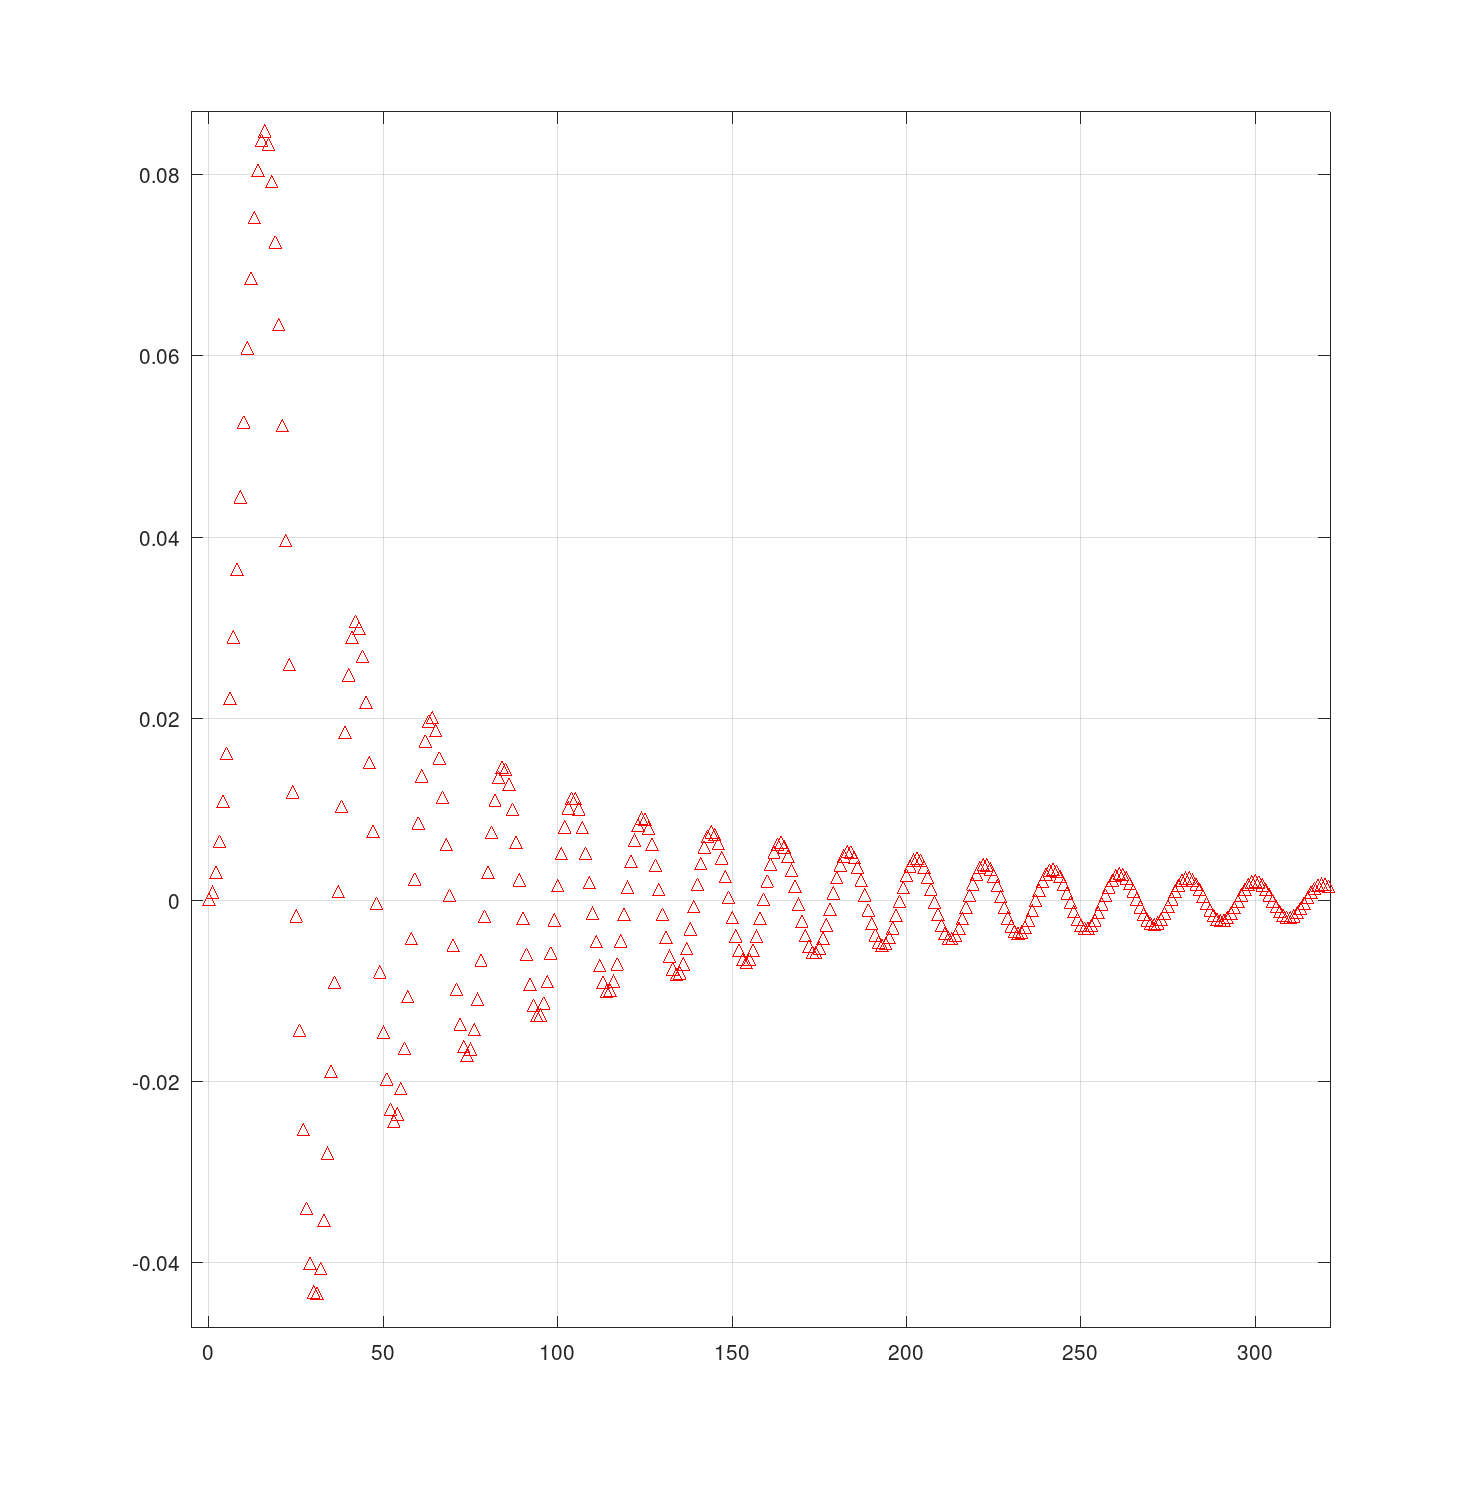
\includegraphics[width=0.52\textwidth]{../images/03-01-untruncated-ellip.png}
      \caption{Respuesta al impulso TIIR de $H^{2}(z)$ según la Ec. \ref{eq:03-01-H}}
      \label{fig:03-00-hfir+}
    \end{figure}

%%% Local Variables:
%%% mode: latex
%%% TeX-master: "../main"
%%% End:


%%% Local Variables:
%%% mode: latex
%%% TeX-master: "../main"
%%% End:
